% GNUPLOT: LaTeX picture with Postscript
\begingroup
  \makeatletter
  \providecommand\color[2][]{%
    \GenericError{(gnuplot) \space\space\space\@spaces}{%
      Package color not loaded in conjunction with
      terminal option `colourtext'%
    }{See the gnuplot documentation for explanation.%
    }{Either use 'blacktext' in gnuplot or load the package
      color.sty in LaTeX.}%
    \renewcommand\color[2][]{}%
  }%
  \providecommand\includegraphics[2][]{%
    \GenericError{(gnuplot) \space\space\space\@spaces}{%
      Package graphicx or graphics not loaded%
    }{See the gnuplot documentation for explanation.%
    }{The gnuplot epslatex terminal needs graphicx.sty or graphics.sty.}%
    \renewcommand\includegraphics[2][]{}%
  }%
  \providecommand\rotatebox[2]{#2}%
  \@ifundefined{ifGPcolor}{%
    \newif\ifGPcolor
    \GPcolortrue
  }{}%
  \@ifundefined{ifGPblacktext}{%
    \newif\ifGPblacktext
    \GPblacktexttrue
  }{}%
  % define a \g@addto@macro without @ in the name:
  \let\gplgaddtomacro\g@addto@macro
  % define empty templates for all commands taking text:
  \gdef\gplbacktext{}%
  \gdef\gplfronttext{}%
  \makeatother
  \ifGPblacktext
    % no textcolor at all
    \def\colorrgb#1{}%
    \def\colorgray#1{}%
  \else
    % gray or color?
    \ifGPcolor
      \def\colorrgb#1{\color[rgb]{#1}}%
      \def\colorgray#1{\color[gray]{#1}}%
      \expandafter\def\csname LTw\endcsname{\color{white}}%
      \expandafter\def\csname LTb\endcsname{\color{black}}%
      \expandafter\def\csname LTa\endcsname{\color{black}}%
      \expandafter\def\csname LT0\endcsname{\color[rgb]{1,0,0}}%
      \expandafter\def\csname LT1\endcsname{\color[rgb]{0,1,0}}%
      \expandafter\def\csname LT2\endcsname{\color[rgb]{0,0,1}}%
      \expandafter\def\csname LT3\endcsname{\color[rgb]{1,0,1}}%
      \expandafter\def\csname LT4\endcsname{\color[rgb]{0,1,1}}%
      \expandafter\def\csname LT5\endcsname{\color[rgb]{1,1,0}}%
      \expandafter\def\csname LT6\endcsname{\color[rgb]{0,0,0}}%
      \expandafter\def\csname LT7\endcsname{\color[rgb]{1,0.3,0}}%
      \expandafter\def\csname LT8\endcsname{\color[rgb]{0.5,0.5,0.5}}%
    \else
      % gray
      \def\colorrgb#1{\color{black}}%
      \def\colorgray#1{\color[gray]{#1}}%
      \expandafter\def\csname LTw\endcsname{\color{white}}%
      \expandafter\def\csname LTb\endcsname{\color{black}}%
      \expandafter\def\csname LTa\endcsname{\color{black}}%
      \expandafter\def\csname LT0\endcsname{\color{black}}%
      \expandafter\def\csname LT1\endcsname{\color{black}}%
      \expandafter\def\csname LT2\endcsname{\color{black}}%
      \expandafter\def\csname LT3\endcsname{\color{black}}%
      \expandafter\def\csname LT4\endcsname{\color{black}}%
      \expandafter\def\csname LT5\endcsname{\color{black}}%
      \expandafter\def\csname LT6\endcsname{\color{black}}%
      \expandafter\def\csname LT7\endcsname{\color{black}}%
      \expandafter\def\csname LT8\endcsname{\color{black}}%
    \fi
  \fi
    \setlength{\unitlength}{0.0500bp}%
    \ifx\gptboxheight\undefined%
      \newlength{\gptboxheight}%
      \newlength{\gptboxwidth}%
      \newsavebox{\gptboxtext}%
    \fi%
    \setlength{\fboxrule}{0.5pt}%
    \setlength{\fboxsep}{1pt}%
\begin{picture}(4520.00,3400.00)%
    \gplgaddtomacro\gplbacktext{%
      \csname LTb\endcsname%
      \put(645,781){\makebox(0,0)[r]{\strut{}$10^3$}}%
      \csname LTb\endcsname%
      \put(645,3195){\makebox(0,0)[r]{\strut{}$10^4$}}%
      \csname LTb\endcsname%
      \put(747,595){\makebox(0,0){\strut{}$10^{14}$}}%
      \csname LTb\endcsname%
      \put(1309,595){\makebox(0,0){\strut{}$10^{15}$}}%
      \csname LTb\endcsname%
      \put(1871,595){\makebox(0,0){\strut{}$10^{16}$}}%
      \csname LTb\endcsname%
      \put(2434,595){\makebox(0,0){\strut{}$10^{17}$}}%
      \csname LTb\endcsname%
      \put(2996,595){\makebox(0,0){\strut{}$10^{18}$}}%
      \csname LTb\endcsname%
      \put(3558,595){\makebox(0,0){\strut{}$10^{19}$}}%
      \csname LTb\endcsname%
      \put(4120,595){\makebox(0,0){\strut{}$10^{20}$}}%
    }%
    \gplgaddtomacro\gplfronttext{%
      \csname LTb\endcsname%
      \put(144,1988){\rotatebox{-270}{\makebox(0,0){\strut{}Mobility $\mu$ ($\frac{cm^2}{Vs}$)}}}%
      \csname LTb\endcsname%
      \put(4305,1988){\rotatebox{-270}{\makebox(0,0){\strut{}}}}%
      \csname LTb\endcsname%
      \put(2433,316){\makebox(0,0){\strut{}Electron density n ($cm^{-3}$)}}%
      \csname LTb\endcsname%
      \put(2433,3102){\makebox(0,0){\strut{}}}%
      \csname LTb\endcsname%
      \put(2433,3101){\makebox(0,0){\strut{}}}%
      \csname LTb\endcsname%
      \put(237,93){\makebox(0,0)[l]{\strut{}}}%
      \csname LTb\endcsname%
      \put(2147,1320){\makebox(0,0){\strut{}}}%
      \csname LTb\endcsname%
      \put(1535,1320){\makebox(0,0)[l]{\strut{}$\mu_{tot}$}}%
      \csname LTb\endcsname%
      \put(1535,1134){\makebox(0,0)[l]{\strut{}$\mu_{Lit,1}$}}%
      \csname LTb\endcsname%
      \put(1535,948){\makebox(0,0)[l]{\strut{}$\mu_{Lit,2}$}}%
      \csname LTb\endcsname%
      \put(2833,1320){\makebox(0,0)[l]{\strut{}$\mu_{Lit,3}$}}%
      \csname LTb\endcsname%
      \put(2833,1134){\makebox(0,0)[l]{\strut{}$\mu_{Lit,4}$}}%
      \csname LTb\endcsname%
      \put(2833,948){\makebox(0,0)[l]{\strut{}$\mu_{Lit,5}$}}%
    }%
    \gplbacktext
    \put(0,0){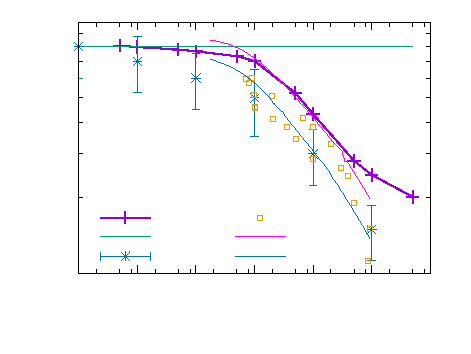
\includegraphics{n-mu-comp-Moore}}%
    \gplfronttext
  \end{picture}%
\endgroup
